\documentclass[UTF8]{beamer}
\usepackage{graphicx, color}
\usepackage{algorithm2e}
\usepackage{zhspacing}
\usepackage{amsmath}
\usepackage{tikz}
\usetikzlibrary{shapes,arrows}

% Define block styles
\tikzstyle{decision} = [diamond, draw, fill=blue!20,
    text width=4.5em, text badly centered, node distance=3cm, inner sep=0pt]
\tikzstyle{block} = [rectangle, draw, fill=blue!20,
    text width=5em, text centered, rounded corners, minimum height=3em]
\tikzstyle{line} = [draw, -latex']
\tikzstyle{cloud} = [draw, ellipse,fill=red!20, node distance=3cm,
    minimum height=2em]

\usepackage{underscore}
\usetheme{JuanLesPins}
\usepackage{fontspec}
\setsansfont{Microsoft YaHei}

\usepackage{enumerate}

\AtBeginSection[]{
  \frame{
    \frametitle{Next}
    \tableofcontents[currentsection, subsectionstyle=show/shaded/hide]
  }
}

\AtBeginSubsection[]{
  \frame{
    \frametitle{Next}
    \tableofcontents[currentsubsection]
  }
}

\title{C in Bioinformatics}

\subtitle{Tools and Projects}

\author{Gang Chen\\ chengang@genomics.cn}

\logo{
\includegraphics[width=1.3cm]{bgi-logo.png}
\includegraphics[width=2.5cm]{cuhklogo.png}}
\date{\today}




\begin{document}


\begin{frame}
\titlepage
\end{frame}
\begin{frame}[t]\frametitle{Outline}
\tableofcontents[hideallsubsections]
\end{frame}

\section{A project: Sequence Alignment in C}

\subsection{Smith-Waterman Algorithm}
\begin{frame}[t]{Overview}
\begin{block}{Smith-Waterman Algorithm}
  The algorithm is proposed by Temple F. Smith and Michael S. Waterman to
  perform local sequence alignment.
\end{block}

\begin{block}{News}
  Michael Waterman has become the first honorary professor of the Chinese
  University of Hong Kong, Shenzhen

  http://www.cuhk.edu.cn/News/142.html
\end{block}

\end{frame}
%--- Next Frame ---%

\begin{frame}[t]{Design}
\begin{columns}
  \begin{column}{.5\textwidth}
\begin{block}{I/O}
  \begin{itemize}
    \item Input: Two sequences: two string;
    \item Output: alignment results;
  \end{itemize}
\end{block}
\end{column}

\begin{column}{.5\textwidth}
\begin{block}{Files}
  \begin{itemize}
    \item swa.h: constant and function declarations;
    \item swa.c: function definitions;
    \item Makefile: ?
  \end{itemize}
\end{block}
\end{column}
\end{columns}
\end{frame}
%--- Next Frame ---%

\subsection{Implementation}
\begin{frame}[t]{swa.h}
  see swa/swa.h
\end{frame}
%--- Next Frame ---%

\begin{frame}[t]{swa.c}
  see swa/swa.c
\end{frame}
%--- Next Frame ---%

\begin{frame}[t]{compile and run}
  gcc swa.c -o swa
  ./swa
\end{frame}
%--- Next Frame ---%

\subsection{Project Management: Makefile}

\begin{frame}[t]{GNU Make}
\begin{block}{GNU Make}
  GNU Make is a tool which controls the generation of executables and other
  non-source files of a program from the program's source files.
\end{block}
\begin{block}{Website}
  http://www.gnu.org/software/make/
\end{block}
\end{frame}
%--- Next Frame ---%

\begin{frame}[t]{Makefile for swa}
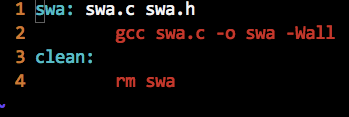
\includegraphics[width=\textwidth]{swamakefile.png}
\end{frame}
%--- Next Frame ---%

\begin{frame}[t]{Tutorials on Makefile}
\begin{itemize}
  \item Tutorial in English: http://makepp.sourceforge.net/
  \item Official Manual: http://www.gnu.org/software/make/manual/make.html
  \item 跟我一起写Makefile:http://blog.csdn.net/haoel/article/details/2886\\
  http://coolshell.cn
\end{itemize}
\end{frame}
%--- Next Frame ---%

\begin{frame}[t]
  \centerline{
\includegraphics[width=.8\textwidth]{baba.png}}
\end{frame}
%--- Next Frame ---%

\begin{frame}[t]{Project Management}
  \begin{itemize}
    \item Source Version Control: git and github;
    \item Generation of Makefile: automake
    \item Documentation: Markdown
  \end{itemize}
\end{frame}
%--- Next Frame ---%

\begin{frame}[t]{Git}
    \begin{itemize}
        \item Git: \url{http://www.git-scm.com/}
        \item SourceTree: \url{https://www.sourcetreeapp.com/}
        \item GitHub Desktop: \url{https://desktop.github.com/}
        \item How to get the latest sources of GNBF5010?
    \end{itemize}
\end{frame}
%--- Next Frame ---%

\section{Bioinformatics Software in C}
\subsection{seqtk}
\begin{frame}
  \frametitle{Overview}
  \begin{block}{seqtk}
    Toolkit for processing sequences in FASTA/Q formats.
  \end{block}
  \begin{block}{Source Codes}
    https://github.com/lh3/seqtk
  \end{block}
\end{frame}

\begin{frame}[t]{Files}
\begin{itemize}
  \item Makefile
  \item README.md
  \item khash.h
  \item kseq.h
  \item ksort.h
  \item kstring.h
  \item ksw.c
  \item ksq.h
  \item kvec.h
  \item seqtk.c
  \item trimadap.c
\end{itemize}
\end{frame}
%--- Next Frame ---%

\begin{frame}[t, fragile]{Compile and Run}
\begin{verbatim}
  make
\end{verbatim}

\begin{verbatim}
  ./seqtk
\end{verbatim}
\end{frame}
%--- Next Frame ---%

\begin{frame}[t]{How to read the codes?}
\begin{block}{Makefile}
  For most C/C++ projects, the best start point to understand the codes is the
  Makefile.
\end{block}

\begin{block}{Why?}
  We have to define the relationship between all source files and executable
  files in the Makefile.
\end{block}

\end{frame}
%--- Next Frame ---%

\begin{frame}[t]{Makefile}
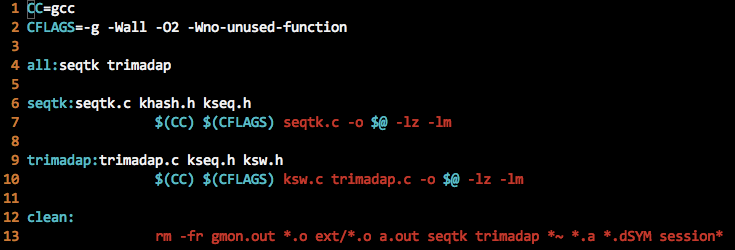
\includegraphics[width=\textwidth]{seqtkmakefile.png}
\end{frame}
%--- Next Frame ---%

\begin{frame}[t]{seqtk.c}
  see seqtk-master/seqtk.c
\end{frame}
%--- Next Frame ---%

\begin{frame}[t, fragile]{Convert FASTQ to FASTA}
\begin{verbatim}
  ./seqtk seq seq.fq > seq.fa
\end{verbatim}
\begin{block}{Data}
  http://trace.ncbi.nlm.nih.gov/Traces/sra/?run=SRR357733
\end{block}
\end{frame}
%--- Next Frame ---%

\begin{frame}[t]{main and stk_seq functions}
  \begin{itemize}
    \item main: see seqtk-master/seqtk.c:1371
    \item stk_seq: see seqtk-master/seqtk.c:1106
  \end{itemize}
\end{frame}
%--- Next Frame ---%

\begin{frame}[t]{Summary}
  \begin{itemize}
    \item Makefile can help us understand source codes;
    \item Typically, declarations are put in header files
    \item and implementation are put in source files;
  \end{itemize}
\end{frame}
%--- Next Frame ---%

\subsection{bwa}
\begin{frame}[t]{Overview}
BWA is a software package for mapping DNA sequences against a large reference
genome, such as the human genome. It consists of three algorithms:
\begin{itemize}
\item BWA-backtrack:designed for Illumina sequence reads up to 100bp;
\item BWA-SW: 70bp to a few megabase;
\item BWA-MEM: 70bp to a few megabase, faster and more accurate;
\end{itemize}
\end{frame}
%--- Next Frame ---%


\begin{frame}[t]{Makefile}
  see bwa-master/Makefile
\end{frame}
%--- Next Frame ---%

\begin{frame}[t]{main function}
  \begin{itemize}
    \item see bwa-master/main.c:60
    \item Call main_mem: bwa-master/main.c:83
    \item main_mem declaration: bwa-master/main.c:24
    \pause\item Where is the function definition?
  \end{itemize}

\end{frame}
%--- Next Frame ---%

\begin{frame}[t]{main_mem function}
\begin{itemize}
  \item Makefile
  \item bwamem.c, bwamem.h \ldots
  \pause \item fastmap.c
\end{itemize}
\end{frame}
%--- Next Frame ---%

\subsection{libsvm}

\begin{frame}[t]{Overview}
\begin{block}{LIBSVM}
  LIBSVM is an integrated software for support vector
  classification(C-SVC, nu-SVC), regression (epsilon-SVR, nu-SVR) and
  distribution estimation (one-class SVM).
\end{block}

\begin{block}{Website}
  http://www.csie.ntu.edu.tw/~cjlin/libsvm/
\end{block}
\end{frame}
%--- Next Frame ---%

\begin{frame}[t]{Overview of Codes}
  \begin{block}{Source Codes}
    \begin{itemize}
      \item A mixture of C and C++;
      \item All C codes are compiled by using C++ compiler;
      \item C++ is used as a C with class and template;
    \end{itemize}
  \end{block}
\end{frame}
%--- Next Frame ---%

\begin{frame}[t]{Makefile}
  see libsvm-3.18/Makefile
\end{frame}
%--- Next Frame ---%

\begin{frame}[t]{svm-train.c}
  \begin{itemize}
    \item main function is definied in svm-train.c
    \item structs are defined in svm.h
    \item functions are declared in svm.h and implemented in svm.cpp
    \item classes and methods are declared and implemented in svm.cpp
    \pause \item the coding style is bad.
  \end{itemize}
\end{frame}
%--- Next Frame ---%

\begin{frame}[t]{C and C++}
  \begin{itemize}
    \item C++ is a upgrade of C?
    \item C++ is C with class?
    \item C++ is C with class, template, meta-programming and so on?
    \item What is the relationship between C and C++?
  \end{itemize}
\end{frame}
%--- Next Frame ---%

\begin{frame}[t]{C and C++}
\begin{itemize}
  \item C++ is a new programming languages;
  \item Currently, C++ is compatible with C;
  \item The latest version of C is C99, C11 is in progress;
  \item The latest version of C++ is C++14, C++17 is in progress.
\end{itemize}
\end{frame}
%--- Next Frame ---%

\begin{frame}
  \centerline{\Huge{Thanks!}}
\end{frame}
%--- Next Frame ---%

\end{document}
